% Options for packages loaded elsewhere
\PassOptionsToPackage{unicode}{hyperref}
\PassOptionsToPackage{hyphens}{url}
%
\documentclass[
  english,
  man]{apa6}
\usepackage{lmodern}
\usepackage{amssymb,amsmath}
\usepackage{ifxetex,ifluatex}
\ifnum 0\ifxetex 1\fi\ifluatex 1\fi=0 % if pdftex
  \usepackage[T1]{fontenc}
  \usepackage[utf8]{inputenc}
  \usepackage{textcomp} % provide euro and other symbols
\else % if luatex or xetex
  \usepackage{unicode-math}
  \defaultfontfeatures{Scale=MatchLowercase}
  \defaultfontfeatures[\rmfamily]{Ligatures=TeX,Scale=1}
\fi
% Use upquote if available, for straight quotes in verbatim environments
\IfFileExists{upquote.sty}{\usepackage{upquote}}{}
\IfFileExists{microtype.sty}{% use microtype if available
  \usepackage[]{microtype}
  \UseMicrotypeSet[protrusion]{basicmath} % disable protrusion for tt fonts
}{}
\makeatletter
\@ifundefined{KOMAClassName}{% if non-KOMA class
  \IfFileExists{parskip.sty}{%
    \usepackage{parskip}
  }{% else
    \setlength{\parindent}{0pt}
    \setlength{\parskip}{6pt plus 2pt minus 1pt}}
}{% if KOMA class
  \KOMAoptions{parskip=half}}
\makeatother
\usepackage{xcolor}
\IfFileExists{xurl.sty}{\usepackage{xurl}}{} % add URL line breaks if available
\IfFileExists{bookmark.sty}{\usepackage{bookmark}}{\usepackage{hyperref}}
\hypersetup{
  pdftitle={A Phoneme-weighted Levenshtein Distance: A Measure of Cross-linguistic Phonological Similarity},
  pdfauthor={First Author1 \& Second Author1,2},
  pdflang={en-EN},
  pdfkeywords={keywords},
  hidelinks,
  pdfcreator={LaTeX via pandoc}}
\urlstyle{same} % disable monospaced font for URLs
\usepackage{graphicx,grffile}
\makeatletter
\def\maxwidth{\ifdim\Gin@nat@width>\linewidth\linewidth\else\Gin@nat@width\fi}
\def\maxheight{\ifdim\Gin@nat@height>\textheight\textheight\else\Gin@nat@height\fi}
\makeatother
% Scale images if necessary, so that they will not overflow the page
% margins by default, and it is still possible to overwrite the defaults
% using explicit options in \includegraphics[width, height, ...]{}
\setkeys{Gin}{width=\maxwidth,height=\maxheight,keepaspectratio}
% Set default figure placement to htbp
\makeatletter
\def\fps@figure{htbp}
\makeatother
\setlength{\emergencystretch}{3em} % prevent overfull lines
\providecommand{\tightlist}{%
  \setlength{\itemsep}{0pt}\setlength{\parskip}{0pt}}
\setcounter{secnumdepth}{-\maxdimen} % remove section numbering
% Make \paragraph and \subparagraph free-standing
\ifx\paragraph\undefined\else
  \let\oldparagraph\paragraph
  \renewcommand{\paragraph}[1]{\oldparagraph{#1}\mbox{}}
\fi
\ifx\subparagraph\undefined\else
  \let\oldsubparagraph\subparagraph
  \renewcommand{\subparagraph}[1]{\oldsubparagraph{#1}\mbox{}}
\fi
% Manuscript styling
\usepackage{upgreek}
\captionsetup{font=singlespacing,justification=justified}

% Table formatting
\usepackage{longtable}
\usepackage{lscape}
% \usepackage[counterclockwise]{rotating}   % Landscape page setup for large tables
\usepackage{multirow}		% Table styling
\usepackage{tabularx}		% Control Column width
\usepackage[flushleft]{threeparttable}	% Allows for three part tables with a specified notes section
\usepackage{threeparttablex}            % Lets threeparttable work with longtable

% Create new environments so endfloat can handle them
% \newenvironment{ltable}
%   {\begin{landscape}\begin{center}\begin{threeparttable}}
%   {\end{threeparttable}\end{center}\end{landscape}}
\newenvironment{lltable}{\begin{landscape}\begin{center}\begin{ThreePartTable}}{\end{ThreePartTable}\end{center}\end{landscape}}

% Enables adjusting longtable caption width to table width
% Solution found at http://golatex.de/longtable-mit-caption-so-breit-wie-die-tabelle-t15767.html
\makeatletter
\newcommand\LastLTentrywidth{1em}
\newlength\longtablewidth
\setlength{\longtablewidth}{1in}
\newcommand{\getlongtablewidth}{\begingroup \ifcsname LT@\roman{LT@tables}\endcsname \global\longtablewidth=0pt \renewcommand{\LT@entry}[2]{\global\advance\longtablewidth by ##2\relax\gdef\LastLTentrywidth{##2}}\@nameuse{LT@\roman{LT@tables}} \fi \endgroup}

% \setlength{\parindent}{0.5in}
% \setlength{\parskip}{0pt plus 0pt minus 0pt}

% \usepackage{etoolbox}
\makeatletter
\patchcmd{\HyOrg@maketitle}
  {\section{\normalfont\normalsize\abstractname}}
  {\section*{\normalfont\normalsize\abstractname}}
  {}{\typeout{Failed to patch abstract.}}
\patchcmd{\HyOrg@maketitle}
  {\section{\protect\normalfont{\@title}}}
  {\section*{\protect\normalfont{\@title}}}
  {}{\typeout{Failed to patch title.}}
\makeatother
\shorttitle{Phoneme-weighted Levenshtein Distance}
\keywords{keywords\newline\indent Word count: X}
\DeclareDelayedFloatFlavor{ThreePartTable}{table}
\DeclareDelayedFloatFlavor{lltable}{table}
\DeclareDelayedFloatFlavor*{longtable}{table}
\makeatletter
\renewcommand{\efloat@iwrite}[1]{\immediate\expandafter\protected@write\csname efloat@post#1\endcsname{}}
\makeatother
\usepackage{lineno}

\linenumbers
\usepackage{csquotes}
\ifxetex
  % Load polyglossia as late as possible: uses bidi with RTL langages (e.g. Hebrew, Arabic)
  \usepackage{polyglossia}
  \setmainlanguage[]{english}
\else
  \usepackage[shorthands=off,main=english]{babel}
\fi

\title{A Phoneme-weighted Levenshtein Distance: A Measure of Cross-linguistic Phonological Similarity}
\author{First Author\textsuperscript{1} \& Second Author\textsuperscript{1,2}}
\date{}


\authornote{

Add complete departmental affiliations for each author here. Each new line herein must be indented, like this line.

Enter author note here.

Correspondence concerning this article should be addressed to First Author, Postal address. E-mail: \href{mailto:my@email.com}{\nolinkurl{my@email.com}}

}

\affiliation{\phantom{0}}

\abstract{
Many studies in bilingualism have explored how form similarity between translation equivalents (i.e.~cognate- ness) impacts language processing. Cognates range from being identical to sharing only a few key features. Although there exists some objective measures of orthographic similarity between word-forms, there is still no representative equivalent for phonological similarity. In infant bilingual research, a measure that reflects perceptual similarity of spoken words as presented in infant-directed speech would be of great value. A widely used metric for word similarity is Levenshtein distance ({\textbf{???}}). This measure calculates word-form similarity by computing the smallest total number of substitutions, insertions and deletions needed to change one word to the other. However, a challenge when defining phonological similarity is that some phonemes (e.g.~{[}k{]} and {[}g{]}) are perceptually more similar than others (e.g.~{[}k{]} and {[}o{]}). The standard Lev- enshtein distance calculation treats each change equally. Thus it often overestimates phonological distance between words. We are developing an adaptation of Levenshtein distance for phonological representations, where edit operations are weighted according to the degree of phonemic feature changes involved, type of change (e.g.~vowel or consonant insertion) and position in the word. To estimate the weights, we are col- lecting behavioural data in an auditory translation elicitation task. Monolingual adult participants with no exposure to the target language will be asked to guess and produce the translations of auditorily-presented words. The only way for participants to guess the correct translation is by mapping the presented unknown phonological form onto the phonology of its known translational equivalent. Cross-linguistic phonological similarity will be operationalised as the probability that participants correctly guess the corresponding trans- lation. The higher the probability, the higher the perceptual similarity. Our weighted similarity metric will provide a useful tool for identifying phonological similarity between words in infant-directed speech.
}



\begin{document}
\maketitle

\hypertarget{methods}{%
\section{Methods}\label{methods}}

\hypertarget{algorithm}{%
\subsection{Algorithm}\label{algorithm}}

\hypertarget{translation-elicitation-task}{%
\subsection{Translation Elicitation task}\label{translation-elicitation-task}}

\hypertarget{participants}{%
\subsubsection{Participants}\label{participants}}

Data collection took place from 04th junio, 2020 to 28th junio, 2020. We collected data from 107 participants (\(M_{age}\) = 21.79, \(SD_{age}\) = 2.41, \(Range_{age}\) = 18-33). 74 participants were British English native speakers living in United Kingdom (49 female), and 74 participants were Spanish native speakers living in Spain (28 female). Participants in UK were recruited via Prolific (5£ compensation) and SONA (compensation in academic credits). Participants in Spain were contacted via announcements in Faculties, and were compensated 5€ or an Amazon voucher for the same value. Participants were asked to complete the experiment in a quiet place with good internet connection. We exluded data from participants that a) self-rated their oral and/or written skills in a second or third language as higher than 4 in a 5-point scale (\emph{n} = 1), b) were diagnosed with a language (\emph{n} = 2)\footnote{We originally planned to exclude participants that reported any visual impairment that glasses would not correct This item was phrased as \enquote{Do you have normal or corrected-to-normal VISION? (Yes/No)} in English, and as \enquote{¿Tienes problemas de VISIÓN que unas gafas o lentes de contacto NO corrijan? (Sí/No)}. However, the proportion of Spanish participants that reported visual impairment was unplausibly large (\emph{n} = 6, 18.18\%). This is possibly due to these participants using glasses dayly and not having read the item until the end, where it is indicated that the use of glasses is considered as normal vision.}, or c) did not contribute more than 80\% of valid trials (\emph{n} = 9).

\hypertarget{procedure}{%
\subsubsection{Procedure}\label{procedure}}

The experiment was implemented online using Psychopy/Pavlovia ({\textbf{???}}). Participants accessed the study from a link provided by Prolific or SONA and completed the experiment from a browser (Chrome or Mozilla). First, participants were informed about the aims of the study and gave informed consent for participating. Second, participants answered a series of questions about their demographic status, their language background, and the set up they were using for completing the study. Third, participants completed the experimental task. Before the task, participants were informed that they would listen to a series of pre-recorded words in Catalan or Spanish (English participants) or only Catalan (Spanish participants). They were instructed to listen to each word, guess its meaning in English (English participants) or Spanish (Spanish participants), and type their answer as soon as possible. English participants were randomly assigned to the list of Catalan or Spanish trials. Spanish participants completed the list of Catalan trials.

\hypertarget{design}{%
\subsubsection{Design}\label{design}}

Each trial started with a yellow fixation dot presented during one second on the center of the screen over a black background. After one second, the audio started playing while the dot remained being displayed until the audio offset. Upon the offset of the fixation point and audio, participants were prompted to write their answer by a \enquote{\textgreater{}} symbol. Typed letters were displayed in the screen in real time to provide visual feed-back to participants. Participants were allowed to correct their answer. Then, participants pressed the RETURN key to start and new trial. We excluded trials where participants did not type an existing word in the correspondent language, or did not type anything at all. Typos were allowed, however. Participants contributed a total of 9536 valid trials (5901 in Catalan, 3635 in Spanish). The task took approximately 15 minutes to be completed.

\hypertarget{stimuli}{%
\subsubsection{Stimuli}\label{stimuli}}

\hypertarget{data-analysis}{%
\subsection{Data analysis}\label{data-analysis}}

We divided participants in three groups: English natives tested in Catalan (ENG-CAT), English natives tested in Spanish (ENG-SPA), and Spanish natives tested in Catalan (SPA-CAT). We analysed the accuracy of responses to each item by calculating the proportion of correct responses across participants, resulting in one data point per item and group. We compared how our similarity score fitted the data in comparison with other measures:total shared phonemes, shared phonemic onset, and orthographical Damerau-Levenshtein distance. We fit several Bayesian linear models ({\textbf{???}}), each including one of the aforementioned variables as predictor, and the proportion of correct reponses as output. Continuous predictors were standadised and categorical predictors were sum-coded ({\textbf{???}}). Missing predictor scores were imputed before fitting the models using multiple imputation ({\textbf{???}}). To test and account for cross-group differences, we included a random intercept for each group. We compared models using Paretho-Smoothed Importance Sampling (PSIS-LOO, ({\textbf{???}})). More information about the models and model comparison can be found in Appendix X.

All analyses were performed in R environment ({\textbf{???}}). We used the \texttt{tidyverse} family of R packages to process data and to generate figures, the \texttt{mice} R package ({\textbf{???}}) to impute missing data, and the \texttt{brms} R package to ({\textbf{???}}) to fit and compare models, which uses the Stan probabilistic programming language language ({\textbf{???}}).

\hypertarget{results}{%
\section{Results}\label{results}}

\hypertarget{posterior-draws}{%
\subsection{Posterior draws}\label{posterior-draws}}

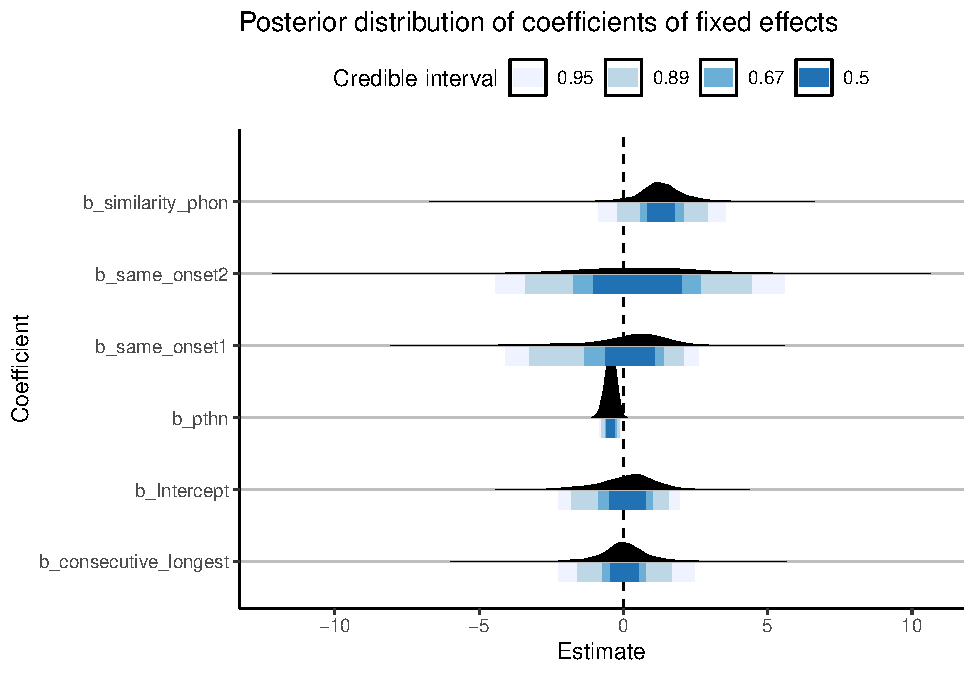
\includegraphics{te_manuscript_files/figure-latex/posterior_draws-1.pdf}

\hypertarget{posterior-predictions}{%
\subsection{Posterior predictions}\label{posterior-predictions}}

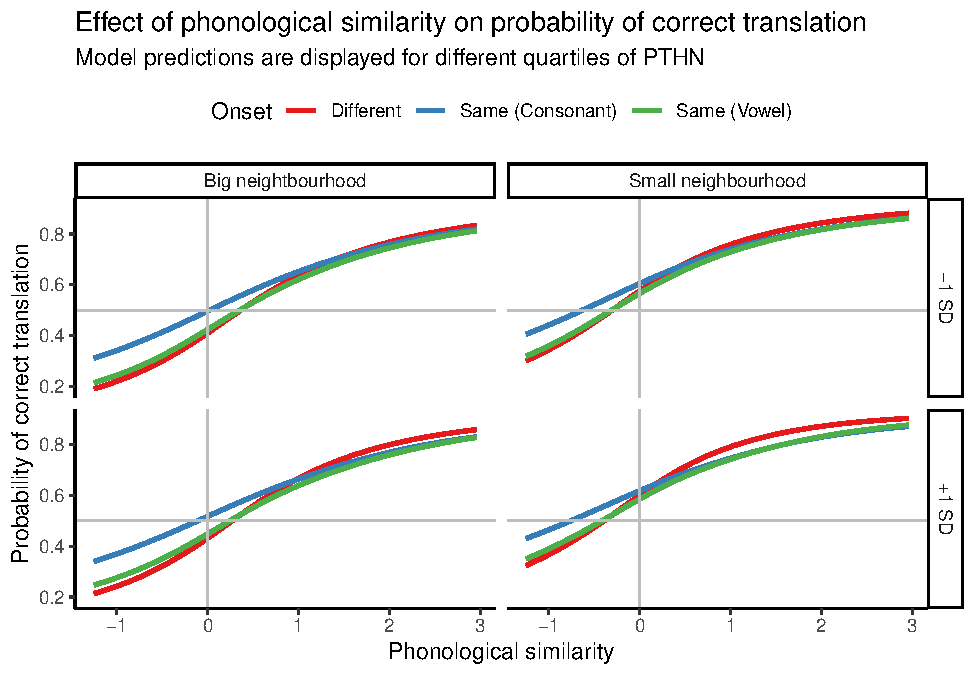
\includegraphics{te_manuscript_files/figure-latex/posterior_predictions-1.pdf}

\hypertarget{random-effects}{%
\subsection{Random effects}\label{random-effects}}

\hypertarget{item-effects}{%
\subsubsection{Item effects}\label{item-effects}}

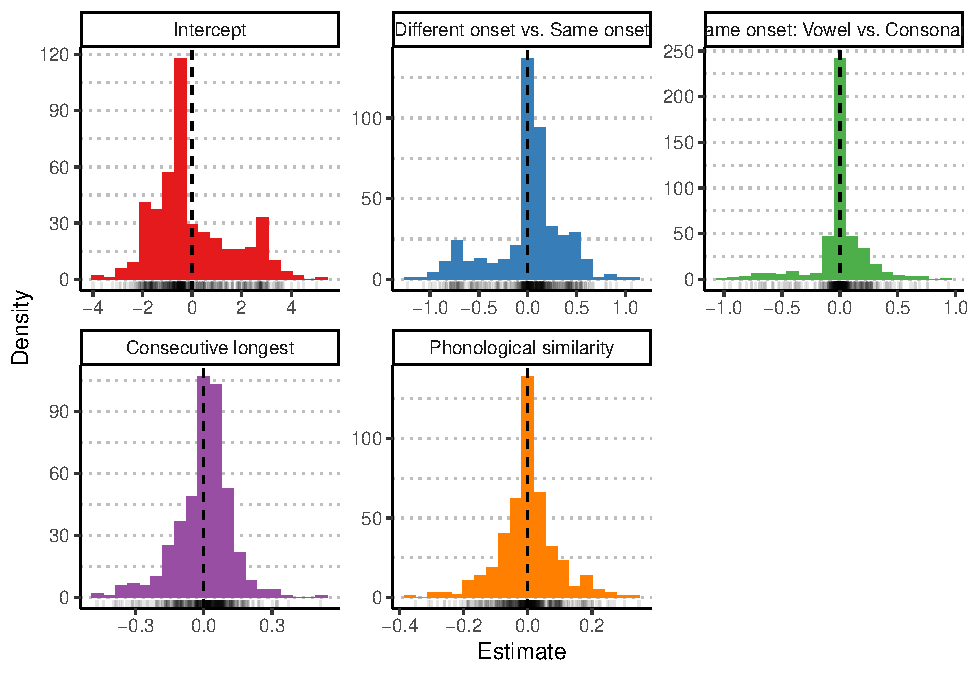
\includegraphics{te_manuscript_files/figure-latex/item_effects-1.pdf}

\hypertarget{group-effects}{%
\subsubsection{Group effects}\label{group-effects}}

\captionsetup[table]{labelformat=empty,skip=1pt}
\begin{longtable}{lrl}
\toprule
Group & SE & 95\% HDI \\ 
\midrule
\multicolumn{1}{l}{Intercept} \\ 
\midrule
ENG-CAT & 1.15 & [-4.27, 0.09] \\ 
ENG-SPA & 1.08 & [-4.05, 0.15] \\ 
SPA-CAT & 0.92 & [-2.87, 0.84] \\ 
\midrule
\multicolumn{1}{l}{Different onset vs. Same onset} \\ 
\midrule
ENG-CAT & 1.73 & [-1.05, 5.49] \\ 
ENG-SPA & 1.62 & [-1.42, 5.09] \\ 
SPA-CAT & 1.49 & [-1.3, 4.56] \\ 
\midrule
\multicolumn{1}{l}{Same onset: Vowel vs. Consonant} \\ 
\midrule
ENG-CAT & 2.58 & [-4.11, 6.94] \\ 
ENG-SPA & 2.59 & [-3.61, 7.29] \\ 
SPA-CAT & 1.98 & [-3.59, 4.64] \\ 
\midrule
\multicolumn{1}{l}{Consecutive longest} \\ 
\midrule
ENG-CAT & 1.09 & [-2.54, 2.18] \\ 
ENG-SPA & 1.13 & [-3.27, 1.59] \\ 
SPA-CAT & 1.11 & [-1.73, 2.94] \\ 
\midrule
\multicolumn{1}{l}{Phonological similarity} \\ 
\midrule
ENG-CAT & 1.05 & [-2.45, 1.96] \\ 
ENG-SPA & 1.04 & [-2.71, 1.69] \\ 
SPA-CAT & 1.10 & [-1.62, 2.87] \\ 
\bottomrule
\end{longtable}

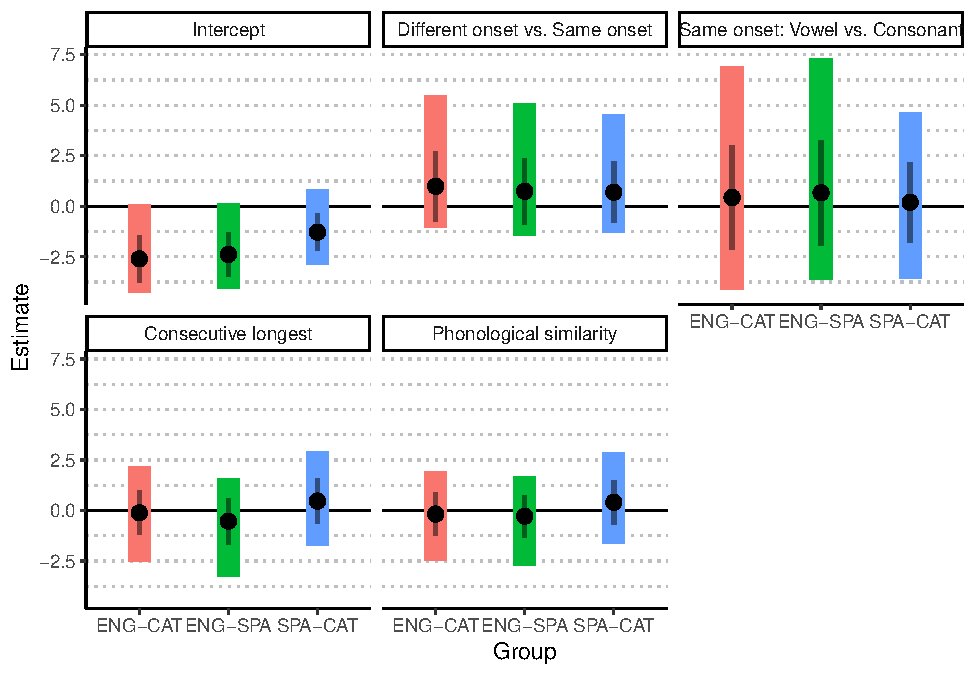
\includegraphics{te_manuscript_files/figure-latex/group_effects-1.pdf}
\#\#\# Correlations

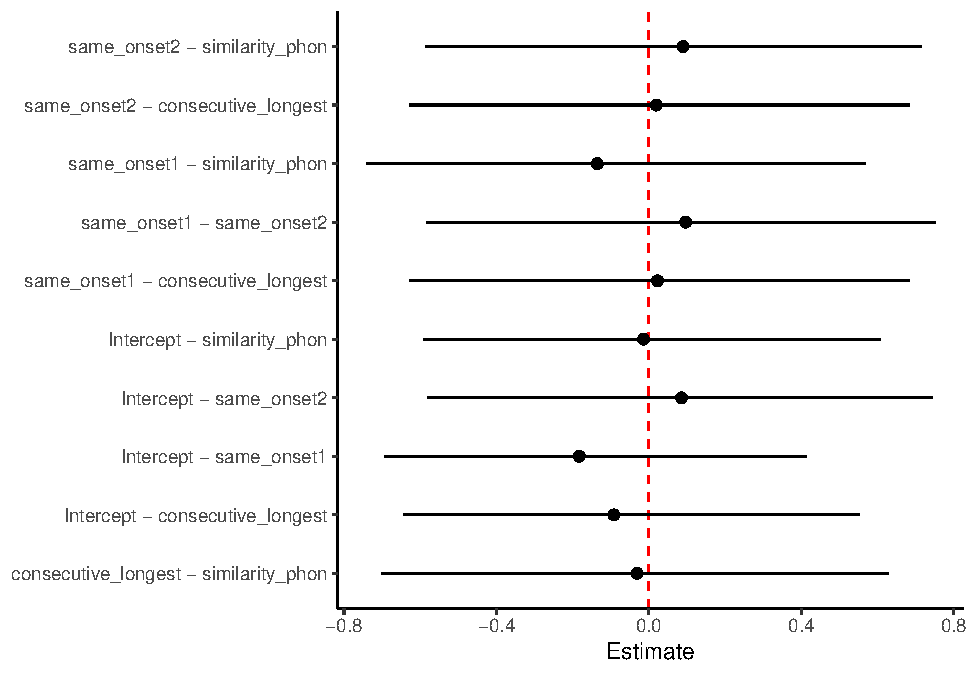
\includegraphics{te_manuscript_files/figure-latex/correlations-1.pdf}

\hypertarget{discussion}{%
\section{Discussion}\label{discussion}}

\newpage

\hypertarget{references}{%
\section{References}\label{references}}

\begingroup
\setlength{\parindent}{-0.5in}
\setlength{\leftskip}{0.5in}

\hypertarget{refs}{}

\endgroup


\end{document}
